\begin{frame}{Ceph - How to expose storage}
\begin{columns}
    \begin{column}{0.47\textwidth}
    \begin{block}{What the Computer sees}
    \begin{figure}
        \centering
        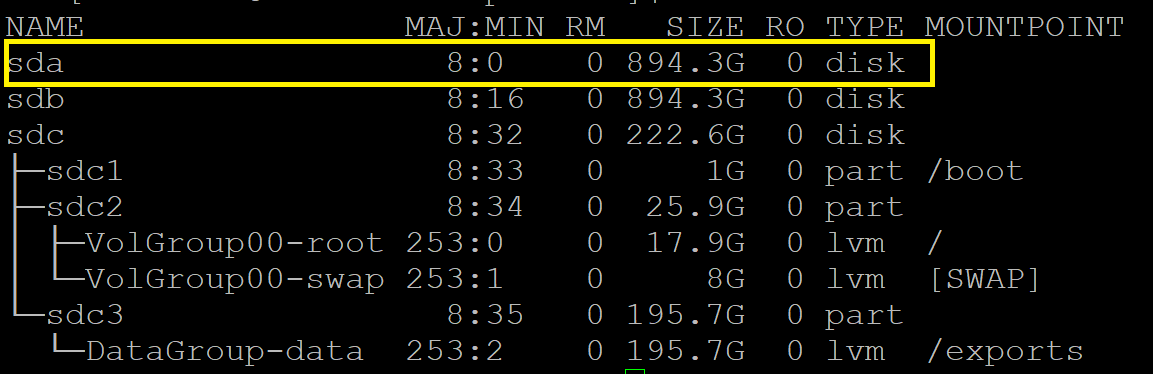
\includegraphics[width=\textwidth,height=0.55\textheight,keepaspectratio]{img/linuxdisk.PNG}
        \caption{Hard drive - sda}
        \label{fig:my_label}
    \end{figure}
    \end{block}
    \end{column}
    \begin{column}{0.47\textwidth}
    \begin{block}{What we see}
    \begin{figure}
        \centering
        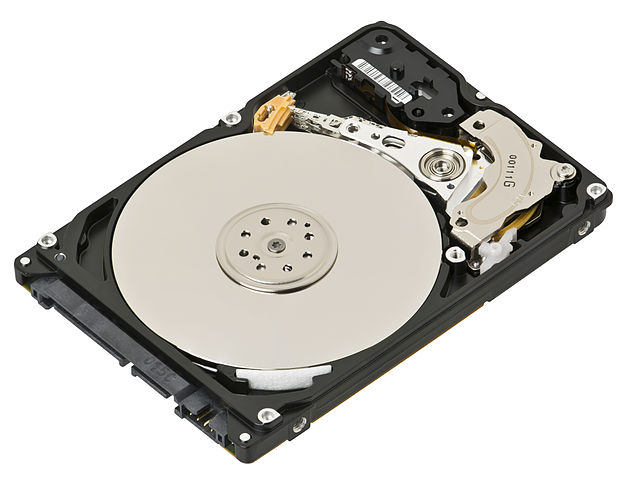
\includegraphics[width=\textwidth,height=0.55\textheight,keepaspectratio]{img/harddrive.jpg}
        \caption{Hard drive - sda}
        \label{fig:my_label}
    \end{figure}
    \end{block}
    \end{column}
\end{columns}
\end{frame}
\note{If we look here we can see that RAM is not exposed in the same way a hard drive is, this is an issue for us, as we want to be use RAM for storage} 

\begin{frame}{Can we make RAM = Disk?}
\begin{columns}
    \begin{column}{0.30\textwidth}
    \begin{figure}
        \centering
        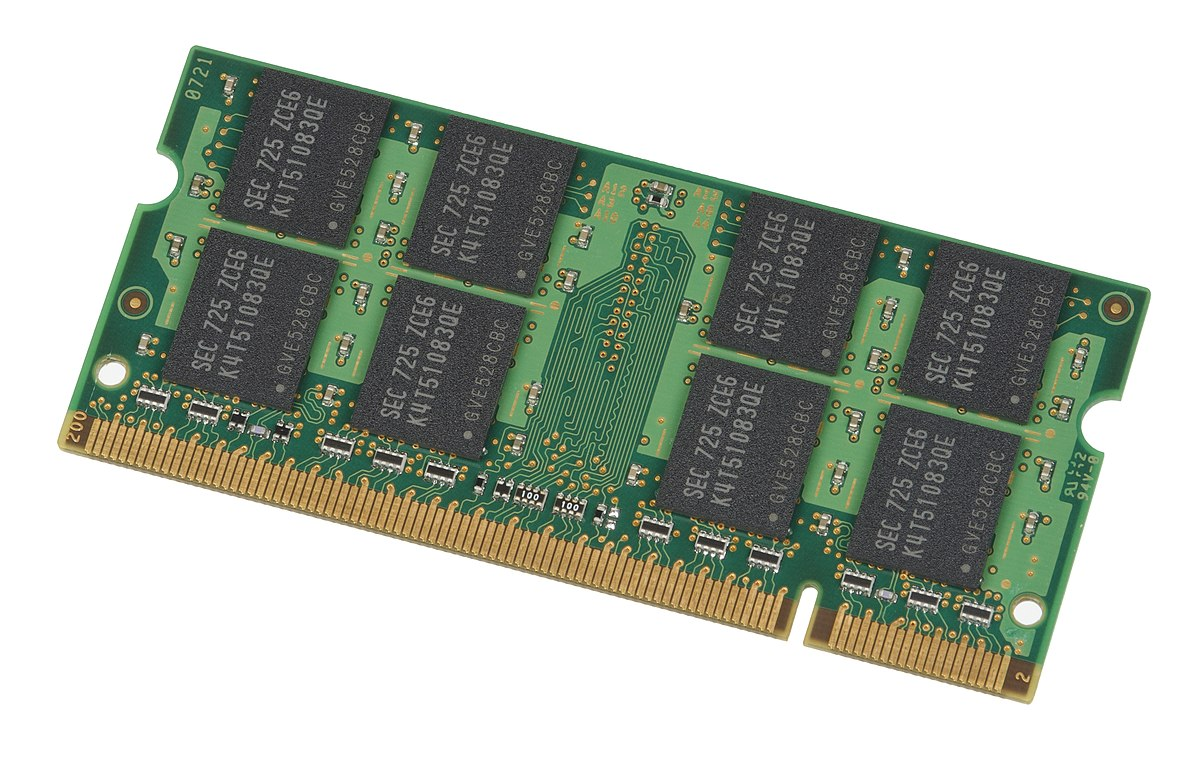
\includegraphics[width=\textwidth,height=0.55\textheight,keepaspectratio]{img/ramdrive.jpg}
        \caption{RAM Drive}
        \label{fig:my_label}
    \end{figure}
    \end{column}
    \begin{column}{0.30\textwidth}
    \begin{figure}
        \centering
        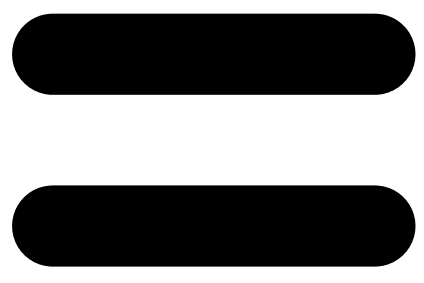
\includegraphics[width=\textwidth,height=0.55\textheight,keepaspectratio]{img/equals (2).png}
        \label{fig:my_label}
    \end{figure}
    \end{column}
    \begin{column}{0.30\textwidth}
    \begin{figure}
        \centering
        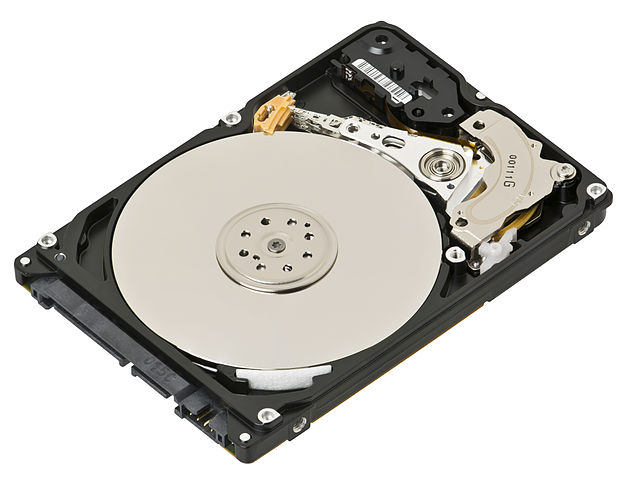
\includegraphics[width=\textwidth,height=0.55\textheight,keepaspectratio]{img/harddrive.jpg}
        \caption{Hard drive - sda}
        \label{fig:my_label}
    \end{figure}
    \end{column}
\end{columns}
\end{frame}
\note{Well the answer is yes and it isn't as difficult as it may seem, in essence we can trick the Linux kernel, into thinking that the RAM drive is actually a block device. How do we do this? Well there are two techniques, you can make your own Linux Module to do it or use the default, or change a pre-existing one to meet your needs.}
\begin{frame}{GRAM VS BRD}
    \begin{figure}
        \centering
        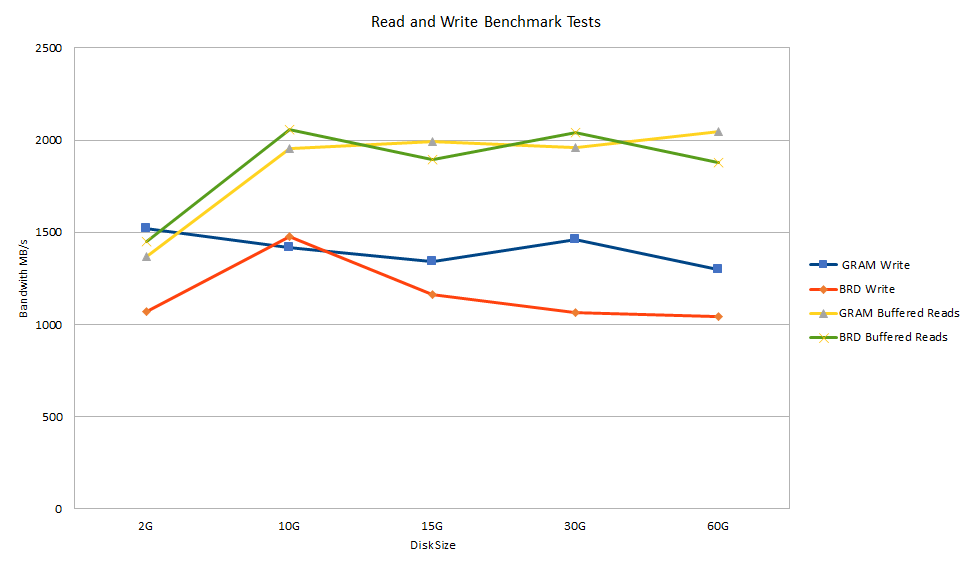
\includegraphics{img/gramVsbrd.png}
        \caption{RAM Block Devices}
        \label{fig:my_label}
    \end{figure}
\end{frame}
\note{So I should give a bit of background GRAM (General RAM) originally started off as my own kernel module, however the performance was to say for the least abysmal, i.e. the speed of a hard drive, due to the way I allocated memory and read and read from it. So after so serious googling I came across ZRAM (Which is a Compression RAM Block Device), so I removed the compression part and gave birth to GRAM. BRD is the default Linux provided block device, what is interesting to see is that BRD is less performant, that's a story for another day.}